\documentclass{article}
\usepackage{times}
\renewcommand{\familydefault}{\sfdefault}

\usepackage[T1]{fontenc}
\usepackage[utf8]{inputenc}
\usepackage[turkish]{babel}
\usepackage{graphicx}       % Grafik eklemek için
\usepackage{caption}        % Resim alt yazısı vs.
\usepackage{booktabs}       % Tablo çizgileri için
\usepackage{amsmath,amssymb}% Matematik
\usepackage{geometry}       % Sayfa ayarları
\usepackage{hyperref}       % Linkler
\usepackage{lipsum}         % Örnek metin
\usepackage{float} % Paketi ekleyin

\geometry{
    a4paper,
    left=25mm,
    right=25mm,
    top=25mm,
    bottom=25mm
}

\title{\textbf{Müşteri Segmentasyonu Projesi}\\
        \large İstanbul Arel Üniversitesi – Veri Madenciliği Dersi Final Projesi}
\author{
    Can Çebi \quad (cancebi21@istanbularel.edu.tr)\\
    Oğuzhan Cem Yücel \quad (oguzhancemyucel21@istanbularel.edu.tr)\\
    \vspace{5pt}
    Danışman/Hoca: Sibel Birtane Akar
}
\date{\today}

\begin{document}

\maketitle

\section{Giriş}

Bu projede, \textbf{Kaggle} ortamında yayınlanan “Customer Segmentation” veri seti kullanılmıştır. Projenin temel amacı, bir müşteri kitlesini ortak özelliklerine göre gruplara (Segmentlere) ayırmaktır. Veri madenciliğinde “müşteri segmentasyonu” (customer segmentation), pazarlama stratejileri ve müşteri yönetimi için önemli bir yaklaşımdır. Segmentasyon, pazarlama kampanyalarının özelleştirilmesine, müşteri memnuniyetinin artırılmasına ve kaynakların verimli kullanılmasına katkı sağlar.

Rapor, \textit{İstanbul Arel Üniversitesi}, \textit{Veri Madenciliği} dersi kapsamında hazırlanmıştır. Burada, hem \textbf{EDA (Keşifsel Veri Analizi)} hem de \textbf{modelleme} adımları sergilenmekte; elde edilen sonuçlar görsellerle birlikte sunulmaktadır.

\section{Veri Seti ve Özellikleri}

Kullanılan veri seti, Kaggle’dan \href{https://www.kaggle.com/datasets/vetrirah/customer}{Customer Segmentation} isimli kaynaktan alınmıştır.

\begin{itemize}
    \item \textbf{Train.csv} dosyası: 8068 satır, 11 sütun
    \item \textbf{Test.csv} dosyası: 2627 satır, 10 sütun
    \item \textbf{sample\_submission.csv}: Örnek Kaggle gönderim formatı (ID, Segmentation)
\end{itemize}

\noindent
Bazı önemli değişkenler şöyledir:
\begin{itemize}
    \item \textbf{ID}: Müşteri ID'si (benzersiz)
    \item \textbf{Gender}: Kadın / Erkek
    \item \textbf{Ever\_Married}: Evli olup olmadığı (Yes/No)
    \item \textbf{Age}: Yaş (sayısal)
    \item \textbf{Graduated}: Üniversite mezunu mu (Yes/No)
    \item \textbf{Profession}: Meslek (Artist, Doctor, Engineer, vb.)
    \item \textbf{Work\_Experience}: Kaç yıllık iş tecrübesine sahip (sayısal)
    \item \textbf{Spending\_Score}: Harcama skoru (Low, Average, High)
    \item \textbf{Family\_Size}: Ailedeki kişi sayısı (sayısal)
    \item \textbf{Var\_1}: Ek bir kategorik sütun (Cat\_1, Cat\_2, vb.)
    \item \textbf{Segmentation}: Hedef değişken (A, B, C, D) (Sadece Train.csv'de)
\end{itemize}

Amaç, Train verisiyle bir model kurup Test verisindeki her müşteri için en olası segmenti (A, B, C, D) tahmin etmektir.

\section{Eksik Değer Analizi ve Veri Hazırlama}

\subsection{Eksik Değerler}

Train ve Test veri setlerinde \textit{Ever\_Married}, \textit{Graduated}, \textit{Profession}, \textit{Work\_Experience}, \textit{Family\_Size}, \textit{Var\_1} gibi sütunlarda eksik değerler gözlenmiştir. Eksik değerlerin veri setindeki dağılımını aşağıdaki Şekil \ref{fig:missing_values} göstermektedir.

\begin{figure}[H]
    \centering
    {\shorthandoff{=}
    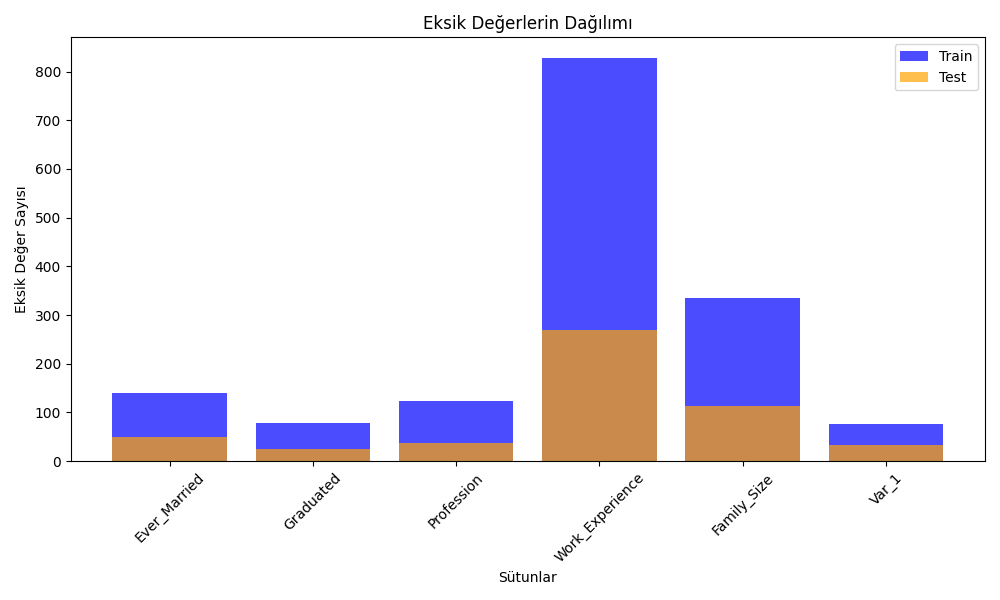
\includegraphics[width=0.5\textwidth]{missing_values_distribution.png}
    }
    \caption{Eksik Değerlerin Dağılımı}
    \label{fig:missing_values}
\end{figure}

Eksik değerleri doldurma stratejisi aşağıdaki gibidir:
\begin{itemize}
    \item Numerik sütunlarda eksik değerler, sütunun ortalama (\textit{mean}) değeri ile doldurulmuştur.
    \item Kategorik sütunlarda eksik değerler, sütunun mod (\textit{mode}, en sık tekrar eden değer) değeri ile doldurulmuştur.
    \item Eksik değerlerin doldurulması sonrası veri setinde artık eksik değer bulunmamaktadır.
\end{itemize}

\subsection{Veri Dönüşümleri}

Veri seti üzerinde yapılan dönüşümler aşağıdaki gibidir:
\begin{itemize}
    \item Kategorik sütunlar (\textit{Gender}, \textit{Ever\_Married}, \textit{Graduated}, \textit{Profession}, \textit{Spending\_Score}, \textit{Var\_1}), makine öğrenmesi yöntemleri için \textbf{Label Encoding} kullanılarak sayısal değerlere dönüştürülmüştür. Örneğin, \textit{Gender} sütununda \textit{Male} değeri 0, \textit{Female} değeri 1 olarak kodlanmıştır.
    \item Sayısal değişkenler (\textit{Age}, \textit{Work\_Experience}, \textit{Family\_Size}), veri setindeki ölçek farklılıklarını gidermek ve algoritmaların daha verimli çalışmasını sağlamak amacıyla \textbf{StandardScaler} ile ölçeklendirilmiştir.
    \item Veri dönüşümleri öncesi ve sonrası değerlerin karşılaştırması Tablo \ref{tab:data_transformation_example}’da sunulmaktadır.
\end{itemize}

\begin{table}[H]
    \centering
    \caption{Veri Dönüşümleri Öncesi ve Sonrası Örnek}
    \label{tab:data_transformation_example}
    \begin{tabular}{|c|c|c|}
        \hline
        \textbf{Değişken} & \textbf{Dönüşüm Öncesi} & \textbf{Dönüşüm Sonrası} \\
        \hline
        Age & 45 & 0.093 \\
        Work\_Experience & 10 & 2.165 \\
        Family\_Size & 4 & 0.756 \\
        \hline
    \end{tabular}
\end{table}

\newpage

\section{EDA (Keşifsel Veri Analizi) ve Bulgular}

Projemizde \textbf{6 adet} grafik oluşturulmuştur:

\begin{itemize}
    \item \textbf{Train Setinde Segmentation Dağılımı}: A, B, C, D segmentlerinin Train verisindeki dağılımını gösterir. Segmentler arasında çok büyük dengesizlik olmadığı görülür.
    \begin{figure}[H]
    \centering
    {\shorthandoff{=}
    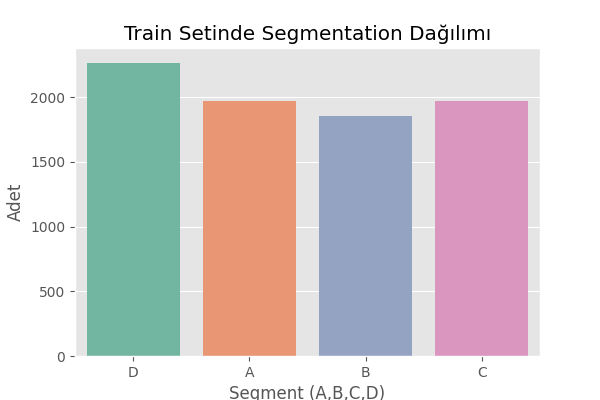
\includegraphics[width=0.5\textwidth]{plot_2024-12-28 15-13-04_0.png}
    }
    \caption{Train Setinde Segmentation Dağılımı}
    \end{figure}
    
    \item \textbf{Cinsiyet Dağılımı (Train)}: Erkek ve kadın müşteri sayısı birbirine yakındır.
    \begin{figure}[H]
    \centering
    {\shorthandoff{=}
    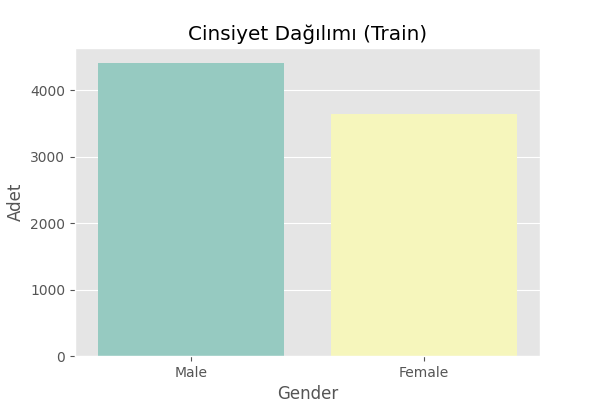
\includegraphics[width=0.5\textwidth]{plot_2024-12-28 15-13-04_1.png}
    }
    \caption{Cinsiyet Dağılımı (Train)}
    \end{figure}

    \item \textbf{Sayısal Değişkenlerin Korelasyon Matrisi}: Age, Work\_Experience, Family\_Size arasındaki korelasyon değerlerinin çok yüksek olmadığı gözlemlenir.
    \begin{figure}[H]
    \centering
    {\shorthandoff{=}
    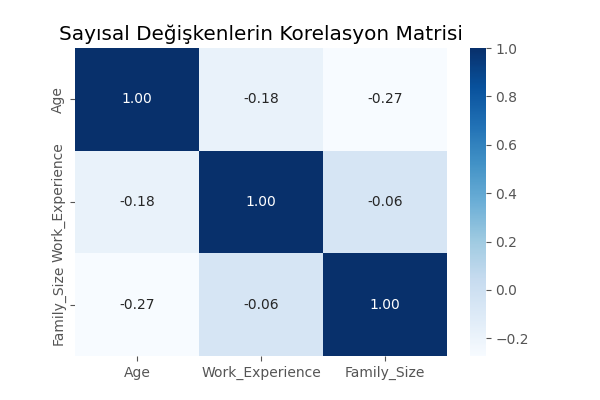
\includegraphics[width=0.5\textwidth]{plot_2024-12-28 15-13-04_2.png}
    }
    \caption{Sayısal Değişkenlerin Korelasyon Matrisi}
    \end{figure}

    \item \textbf{Profession dağılımı Segmentation'a göre}: Bazı meslek gruplarında, belli segmentlerin (A/B/C/D) yoğunlaştığı görülebilir.
    \begin{figure}[H]
    \centering
    {\shorthandoff{=}
    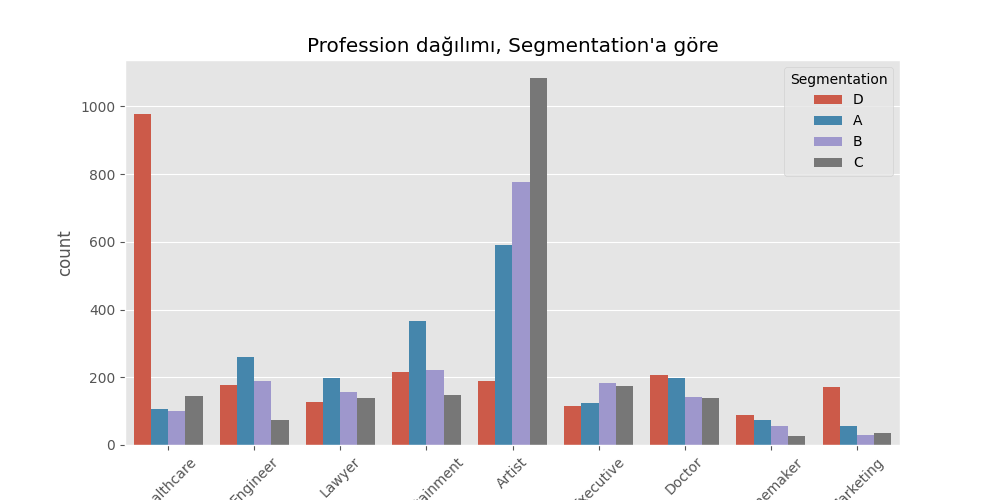
\includegraphics[width=0.5\textwidth]{plot_2024-12-28 15-13-04_3.png}
    }
    \caption{Profession dağılımı Segmentation'a göre}
    \end{figure}
        
    \item \textbf{Confusion Matrix (Validation Set)}: Confusion Matrix, modelin Segmentasyon "3" sınıfında yüksek doğruluk sağladığını, ancak diğer sınıflar arasında karışıklık olduğunu göstermektedir.
    \begin{figure}[H]
    \centering
    {\shorthandoff{=}
    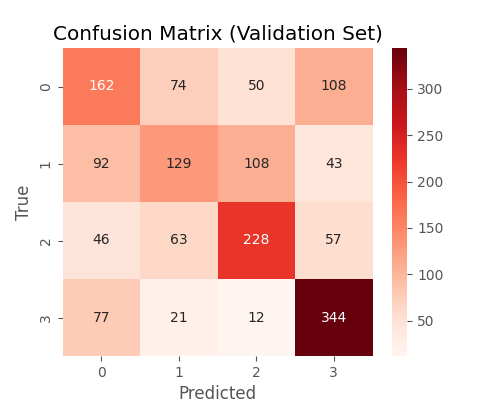
\includegraphics[width=0.5\textwidth]{plot_2024-12-28 15-13-04_4.png}
    }
    \caption{Confusion Matrix (Validation Set)}
    \end{figure}
    
    \item \textbf{Özellik Önem Sıralaması (RandomForest)}: "Age" ve "Profession" özellikleri, segmentasyon tahminlerinde en belirleyici faktörlerdir.
    \begin{figure}[H]
    \centering
    {\shorthandoff{=}
    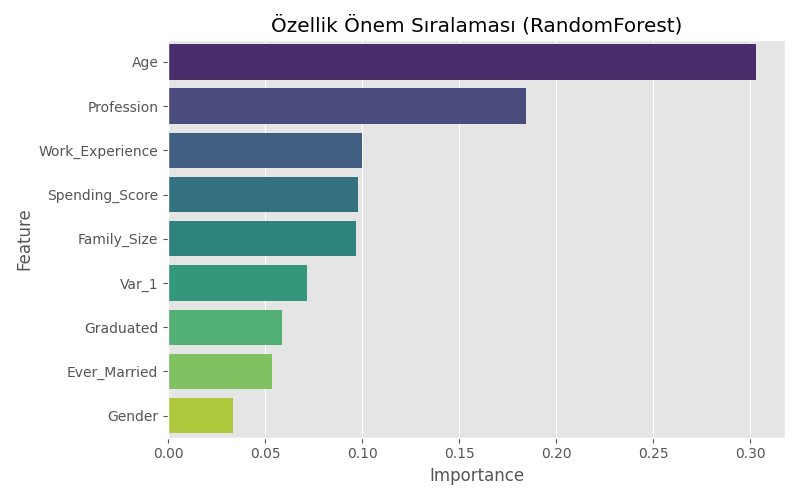
\includegraphics[width=0.5\textwidth]{plot_2024-12-28 15-13-04_5.png}
    }
    \caption{Özellik Önem Sıralaması (RandomForest)}
    \end{figure}

\end{itemize}

\section{Model Kurulumu, Seçimi ve Eğitimi}

\subsection{Model Seçimi}

\textbf{RandomForestClassifier} tercih edilmiştir. Hem kategorik hem de numerik verilerde iyi sonuç verebilmesi ve \textit{ensemble} yaklaşımına sahip olması büyük avantaj sağlamaktadır. \textbf{GridSearchCV} ile:
\begin{itemize}
    \item n\_estimators: [100, 200]
    \item max\_depth: [None, 10, 20]
\end{itemize}
taranmış, en iyi parametreler \{\texttt{max\_depth: 10, n\_estimators: 200}\} olarak bulunmuştur.


\subsection{Eğitim ve Değerlendirme}

Train verisi, \texttt{train\_test\_split} yöntemiyle \%80 eğitim, \%20 doğrulama şeklinde ikiye ayrılmıştır. Değerlendirme metrikleri: \textit{accuracy, precision, recall, f1-score}.

\textbf{Validation Sonuçları (RandomForest, en iyi model)}:

\begin{verbatim}
precision    recall  f1-score   support

0 (A)       0.43      0.41      0.42       394
1 (B)       0.45      0.35      0.39       372
2 (C)       0.57      0.58      0.58       394
3 (D)       0.62      0.76      0.68       454

accuracy                           0.53      1614
macro avg       0.52      0.52      0.52      1614
weighted avg    0.52      0.53      0.53      1614
\end{verbatim}

Doğruluk (\textit{accuracy}) yaklaşık \textbf{\%53}, makro ortalama F1 \textbf{0.52} civarındadır.



Konfüzyon matrisi incelendiğinde, özellikle A ve B segmentleri arasında karışmaların olduğu gözlenmektedir. D segmenti en net ayrışan sınıftır (yüksek recall).

\section{Sonuçların Analizi ve Yorumlanması}

\subsection{Model Başarısı}

Rastgele orman (RandomForest) ile \%53 doğruluk elde edilmiştir. Verisetinin karmaşık yapısı göz önüne alındığında, performans orta seviyededir. Bazı segmentlerde (özellikle B) modelin yanılma payı yüksektir.

\subsection{Hata Analizi}

\begin{itemize}
    \item A-B segmentleri arasında hatalı sınıflandırmalar gözlenir.
    \item D segmenti daha net tespit edilir (yüksek recall).
\end{itemize}
D segmentindeki müşterilerin profile daha tutarlı özellikler sergilediği düşünülebilir.

\subsection{Uygulama Alanları ve Öneriler}

\begin{itemize}
    \item Pazarlama kampanyaları, bu segmente (ör. D) göre özelleştirildiğinde başarı artabilir.
    \item B segmentini iyileştirmek adına ek veri veya farklı özellikler (feature engineering) faydalı olabilir.
\end{itemize}

\section{Sonuçların Raporlanması ve Sunumu}

\subsection{Proje Metrikleri}

\begin{enumerate}
    \item \textbf{Model Seçimi (30 puan)}: RandomForest seçildi, GridSearchCV ile parametreleri belirlendi, doğruluk \%53 civarında.
    \item \textbf{Sonuçların Analizi (35 puan)}: Confusion matrix, precision/recall, F1-skor incelendi. Segmentler arası karışmalar analiz edildi, “B” segmentinde zorluk görüldü.
    \item \textbf{Sonuçların Raporlanması (35 puan)}: 6 adet grafik, tablo ve açıklamalar. Modelin doğruluğu, hata analizi, uygulama önerileri verilmiştir.
\end{enumerate}

\textbf{my\_submission.csv} dosyası, test veri setindeki müşterilerin öngörülen (A, B, C, D) segmentlerini içerir. Firma bu sonuçlardan yararlanarak özelleştirilmiş pazarlama stratejileri geliştirebilir.

\section{Genel Değerlendirme}

\begin{itemize}
    \item Modelin doğruluğu \%53’tür, segmentlerin ayrıştırılma güçlüğü söz konusudur.
    \item Diğer modeller (XGBoost, LightGBM, vb.) veya ek veriyle performans artabilir.
    \item Eksik değer stratejilerinde ve feature engineering aşamalarında yapılacak ek çalışmalarla sonuçlar iyileştirilebilir.
\end{itemize}

\section*{Kaynaklar}
\begin{itemize}
    \item Kaggle “Customer Segmentation” Dataset: \newline \texttt{https://www.kaggle.com/datasets/vetrirah/customer}
    \item Han, J., Kamber, M., \& Pei, J. (2011). \textit{Data Mining: Concepts and Techniques}. Elsevier.
    \item Aggarwal, C. C. (2015). \textit{Data Mining: The Textbook}. Springer.
    \item Scikit-Learn Dokümantasyonu: \texttt{https://scikit-learn.org/stable/}
\end{itemize}

\vspace{15pt}
\noindent
\textbf{Proje Ekibi:}\\
Can Çebi (cancebi21@istanbularel.edu.tr)\\
Oğuzhan Cem Yücel (oguzhancemyucel21@istanbularel.edu.tr)

\vspace{10pt}
\noindent
\textbf{Teşekkürler:} Bu rapor, Veri Madenciliği dersi kapsamında değerli katkı ve yönlendirmeleri için Sibel Birtane Akar hocamıza ve bölüm arkadaşlarımıza ithafen hazırlanmıştır.

\end{document}
